% This is the file in which the begin is



%%%%%%%%%%%%%%%%%%%%%%%%%%%%%%%%%%%%%%%%%%%%%%%%%%SECTION%%%%%%%%%%%%%%%%%%%%%%%%%%%%%%%%%%%%%%%%%%%%%%%%%%
\section{Hindernisse Überkommen}
%%%%%%%%%%%%%%%%%%%%%%%%%%%%%%%%%%%%%%%%%%%%%%%%%%SECTION%%%%%%%%%%%%%%%%%%%%%%%%%%%%%%%%%%%%%%%%%%%%%%%%%%

\begin{frame}[c]{Warum ist Strategie überhaupt wichtig?}
    Mehrere Gründe, vor allem: \\
    \pause
    \begin{itemize}
        \item Das Leben besteht aus lauter Problem
            \pause
        \item Strategisch zu Denken hilft einem Sinnvolle Entscheidungen zu treffen
            \pause
        \item Oder: Mathematische Probleme Strategisch zu betracheten
            \pause
        \item Das 'Spiel Gewinnen'
            \pause
        \item Einen Vorteil haben, der jedem Zugänglich ist
            \pause
        \item Allgemein: Problemstellungen mit Neuen Werkzeugen Bezwingen
    \end{itemize}
\end{frame}


%%%%%%%%%%%%%%%%%%%%%%%%%%%%%%%%%%%%%%%%%%%%%%%%%%SECTION%%%%%%%%%%%%%%%%%%%%%%%%%%%%%%%%%%%%%%%%%%%%%%%%%%
\section{Disclaimer}
%%%%%%%%%%%%%%%%%%%%%%%%%%%%%%%%%%%%%%%%%%%%%%%%%%SECTION%%%%%%%%%%%%%%%%%%%%%%%%%%%%%%%%%%%%%%%%%%%%%%%%%%
\begin{frame}[c]{Disclaimer}
    Ein paar beispiele kommen aus der Welt der Wirtschaft. \\ \pause

    \vfill

    Das heißt aber noch lange nicht, dass sich Strategie nur dort anwenden lässt.
\end{frame}



%%%%%%%%%%%%%%%%%%%%%%%%%%%%%%%%%%%%%%%%%%%%%%%%%%SECTION%%%%%%%%%%%%%%%%%%%%%%%%%%%%%%%%%%%%%%%%%%%%%%%%%%
\section{Mächtigkeit guter Strategie}
%%%%%%%%%%%%%%%%%%%%%%%%%%%%%%%%%%%%%%%%%%%%%%%%%%SECTION%%%%%%%%%%%%%%%%%%%%%%%%%%%%%%%%%%%%%%%%%%%%%%%%%%

\subsection{Napoleon gegen die Briten}

\begin{frame}[c, fragile]{Schlacht von Trafalgar I}
    Napoleon (Villeneuve):
    \begin{itemize}
        \item Frankreich + Spanien
        \item<2-> \verb!   18    +   15   ! Linienschiffe
        \item<2-> \verb!   08    +   00   ! Andere
        \item<3-> Summe: 41 Schiffe
    \end{itemize}

    Lord Nelson:
    \begin{itemize}
        \item England
        \item<2-> 27 Linienschiffe
        \item<2-> 06 Andere
        \item<3-> Summe: 33 Schiffe
    \end{itemize}
    \pause
    \pause
    \pause

    Wer Gewinnt also?
\end{frame}

\begin{frame}{Schlacht von Trafalgar II}
    Aber wie? \\
    \pause
    Traditionelle See-Schlachten: Linienkämpfe \\
    \pause
    Nelsons Plan: \\
    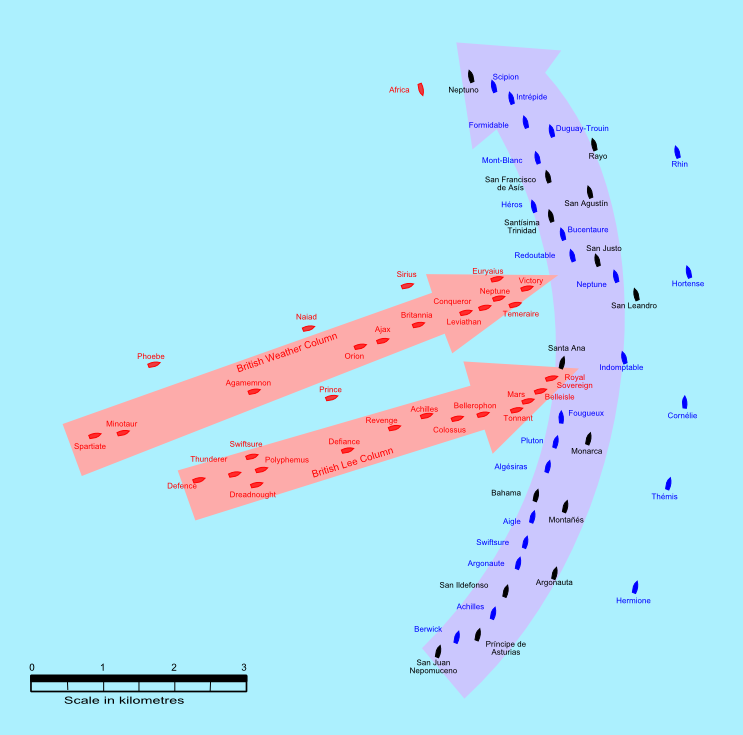
\includegraphics[height=6cm]{strategy/Trafalgar-1200hr.jpg}
\end{frame}

\begin{frame}{Schlacht von Trafalgar III}
    \begin{multicols}{2}
        Verluste für Villeneuve (Napoleon) \\
        Frankreich:
        \begin{itemize}
            \item<2-> 10 Schiffe
            \item<2-> 1 Schiff Zerstört
            \item<3-> 2'218 Tote
            \item<3-> 1'155 Verletzte
            \item<4-> ~4'000 Gefangene
        \end{itemize}
        Spanien:
        \begin{itemize}
            \item<2-> 11 Schiffe
            \item<3-> 1'025 Tote
            \item<3-> 1'383 Verletzte
            \item<4-> ~4'000 Gefangene
        \end{itemize}
        \visible<5> {Summe: 22 Schiffe + 13'781 Außer Gefecht}


        Verluste für die Briten
        \begin{itemize}
            \item<2-> Kein einziges Schiff
            \item<3-> 458 Tote
            \item<3-> 1'208 Verletzte
            \item<5-> Insgesamt: 1'666 Außer Gefecht
        \end{itemize}

        \pause
        \pause
        \pause
        \pause

    \end{multicols}

\end{frame}



\subsection{Steve Jobs Rettet Apple}

\begin{frame}{Steve Jobs Rettet Apple I}
    September 1997. \\
    Apple ist 2 Monate entfernt von Insolvenz. \\
    \pause
    Angebot: \\
    \begin{itemize}
        \item 15 verschiedene Desktop-Rechner
        \item Unglaublich viele Laptops (+ ähnliches)
        \item Mehrere Drucker etc.
        \item 6 Apple-Stores
    \end{itemize}
    \pause

    Was hat er also getan?

\end{frame}

\begin{frame}{Steve Jobs Rettet Apple II}
    \iffinal
    \small
    \fi
    Er hat das Offensichtliche Getan\pause,
    danach gab es:
    \begin{itemize}
        \item 1 Desktop-Rechner
        \item 1 Laptop
        \item Keine Drucker oder ähnliches
        \item 1 Apple Store
        \item viel weniger Entwickler !!
        \item Produktion in Taiwan
        \item Inventarverkleinerung (80\%)
        \item Neuer Web-Store
    \end{itemize}
    \iffinal
    \pause
    Das erschreckende ist, wie viel davon Wirtschafts-101 ist,
    und dennoch Unerwartet war. \\
    \pause
    Außerdem Bat er Bill Gates um 150Millionen
    \fi
\end{frame}

\begin{frame}[c]{Steve Jobs Rettet Apple III}
    \Large
    Was war sein Plan für die Zukunft? \\
    \pause

    Steve Jobs: ``Ich warte auf das nächste große Ding.''

\end{frame}

\subsection{Strategie ist Unerwartet}

\begin{frame}[c]{Strategie ist Unerwartet}
    \Large
    Merke: Allein eine Strategie zu haben kann extrem Mächtig sein.
\end{frame}



%%%%%%%%%%%%%%%%%%%%%%%%%%%%%%%%%%%%%%%%%%%%%%%%%%SECTION%%%%%%%%%%%%%%%%%%%%%%%%%%%%%%%%%%%%%%%%%%%%%%%%%%
\section{Nicht-Strategie}
%%%%%%%%%%%%%%%%%%%%%%%%%%%%%%%%%%%%%%%%%%%%%%%%%%SECTION%%%%%%%%%%%%%%%%%%%%%%%%%%%%%%%%%%%%%%%%%%%%%%%%%%

\subsection{Beispiele für Nicht-Strategie}

\begin{frame}[c]{Beispiele für Nicht-Strategie}
    \begin{itemize}
            \iffinal
        \item Ich werde viele Gute Noten schreiben! \pause
        \item Wir werden Dieses Jahr Erfolgreicher als jeher! \pause
            \fi
        \item Wir werden den Gegner vernichtend Schlagen! \pause
        \item Nicht aufhören, bis man sein Ziel erreicht. \pause
        \item Ich möchte eine Gute Note schreiben. Daher esse ich Kuchen. \pause
        \item Ich möchte eigentlich PI auswendig lernen (, weiß aber nicht wie ich das am Besten mache). \pause
        \item Mithilfe dieser Supercoolen Pi-Kärtchen werden wir Kuchen und die Welt erobern!
    \end{itemize}
\end{frame}

\begin{frame}[c]{Nicht-Strategie}
    \large
    \begin{itemize}
        \item Flauschige Ziele
        \item Die Herausforderung verfehlen
        \item Visionen
        \item Schlechte Strategische Ziele
        \item Inkonsistente Ziele / Aktionen
    \end{itemize}
\end{frame}


\begin{frame}[c]{Flauschige Ziele}
    Buzzword-Bing + Esoterische Konzepte um den Eindruck zu erwecken,
    man Hätte sich darüber Gedanken gemacht.
    \newline
    \newline
    \pause
    Beispiel: Mithilfe dieser Supercoolen Pi-Kärtchen werden wir Kuchen und die Welt erobern! \pause \\
    Buzzwords: Supercool, Pi-Kärtchen, Kuchen, Welt erobern.
\end{frame}


\begin{frame}[c]{Die Herausforderung verfehlen}
    Nicht-Strategie ist nicht in der Lage, die Herausforderung zu Adressieren.
    Wenn man die Herausforderung nicht adressiert \iffinal (sich darum kümmert) \fi, ist es
    nicht möglich die Strategie zu bewerten oder verbessern.
    \newline
    \newline
    \pause
    Beispiel: Nicht aufhören, bis man sein Ziel erreicht. \\ \pause
    Problem: Was ist hier die Herausforderung? wie soll man diese angehen?
\end{frame}


\begin{frame}[c]{Visionen}
    viele 'Strategien' sind nur eine ansammlung an Wünschen die in Erfüllung gehen sollen.
    \newline
    \newline
    \pause
    Beispiel: Ich möchte eigentlich PI auswendig lernen (, weiß aber nicht wie ich das am Besten mache). \\ \pause
    Problem: weiß aber nicht wie ich das am Besten mache
\end{frame}


\begin{frame}[c]{Schlechte Strategische Ziele}
    Strategische Ziele werden meist von einem Höhergestellten festgelegt,
    allerdings sind sie schlecht, wenn sie entweder kritische Zustände
    ignorieren oder Inpraktikabel sind.
    \newline
    \newline
    \pause
    Beispiel: Wir werden den Gegner vernichtend Schlagen! \\ \pause
    Problem: ignoriert evtl. dass der Gegner viel mehr Truppen hat.
\end{frame}


\begin{frame}[c]{Inkonsistente Ziele / Aktionen}
    Strategie ist außerdem nicht Gut, wenn die Ziele sowie die Aktionen im allgemeinen
    nicht Konsistent sind
    \iffinal
    , also sich die Aktionen oder Ziele gegenseitig 'zunichte machen'
    \fi
    .
    \newline
    \newline
    \pause
    Beispiel: Ich möchte eine Gute Note schreiben. Daher esse ich Kuchen. \\ \pause
    Problem: Ziel und Aktion Inkonsistent.
\end{frame}


\subsection{Warum gibt es so viel Nicht-Strategie?}

\begin{frame}[c]{Warum so viel Nicht-Strategie?}
    \Large
    \begin{itemize}
        \item Aktives vermeiden von Analyse \pause
        \item Aktives vermeiden von Wählen zwischen Alternativen \pause
        \item Vorgefertigte Ausfüll-'Strategien' \pause
        \item 'Neue Gedanken'
    \end{itemize}
\end{frame}


\begin{frame}[c]{Ausfüll-Strategie}
    Was ist die VISION:
    \newline
    \newline
    \newline
    Was ist die MISSION:
    \newline
    \newline
    \newline
    Welche WERTE werden Vertreten:
    \newline
    \newline
    \newline
    Was ist die STRATEGIE:
    \newline
    \newline
\end{frame}


\begin{frame}[c]{Ausfüll-Strategie}
    Was ist die VISION:
    \newline
    Gute Noten ohne viel zu lernen
    \newline
    \newline
    Was ist die MISSION:
    \newline
    \newline
    \newline
    Welche WERTE werden Vertreten:
    \newline
    \newline
    \newline
    Was ist die STRATEGIE:
    \newline
    \newline
\end{frame}


\begin{frame}[c]{Ausfüll-Strategie}
    Was ist die VISION:
    \newline
    Gute Noten ohne viel zu lernen
    \newline
    \newline
    Was ist die MISSION:
    \newline
    Die Welt retten
    \newline
    \newline
    Welche WERTE werden Vertreten:
    \newline
    \newline
    \newline
    Was ist die STRATEGIE:
    \newline
    \newline
\end{frame}


\begin{frame}[c]{Ausfüll-Strategie}
    Was ist die VISION:
    \newline
    Gute Noten ohne viel zu lernen
    \newline
    \newline
    Was ist die MISSION:
    \newline
    Die Welt retten
    \newline
    \newline
    Welche WERTE werden Vertreten:
    \newline
    Utilitarismus, Freundliches Miteinander
    \newline
    \newline
    Was ist die STRATEGIE:
    \newline
    \newline
\end{frame}


\begin{frame}[c]{Ausfüll-Strategie}
    Was ist die VISION:
    \newline
    Gute Noten ohne viel zu lernen
    \newline
    \newline
    Was ist die MISSION:
    \newline
    Die Welt retten
    \newline
    \newline
    Welche WERTE werden Vertreten:
    \newline
    Utilitarismus, Freundliches Miteinander
    \newline
    \newline
    Was ist die STRATEGIE:
    \newline
    Hin und wieder ein wenig Lernen.
    \newline
\end{frame}



\begin{frame}[c]{'Neue Gedanken'}
    \LARGE
    Die Idee, dass das einzig nötige um etwas zu schaffen eine Positive Einstellung ist.
    \pause
    \newline
    \newline
    Dem ist leider nicht so.
\end{frame}



